\documentclass[11pt, a4paper]{article}

\usepackage{listings}
\usepackage{subfigure}
\usepackage{graphicx}
\usepackage{titling}
% \usepackage[margin=1.8cm, includefoot]{geometry}
\usepackage{parskip}
\setlength{\parindent}{0cm}
\usepackage{titlesec}
\usepackage{pdfpages}
\usepackage{cleveref}

% Select what to do with todonotes: 
% \usepackage[disable]{todonotes} % notes not showed
\usepackage[draft]{todonotes}   % notes showed

\newlength\longest

\titlespacing\section{0pt}{6pt plus 2pt minus 2pt}{0pt plus 0pt minus 2pt}
\titlespacing\subsection{0pt}{4pt plus 2pt minus 2pt}{0pt plus 0pt minus 2pt}
\newcommand{\subtitle}[1]{
  \posttitle{
    \par\end{center}
    \begin{center}\large#1\end{center}
    \vskip0.5em}
}

\setlength{\droptitle}{-4em}

\newcommand{\cmd}[1]{{\tt #1}}

\begin{document}

\title{Deeva}
\subtitle{Final Report}
\author{Kritaphat Sonsri-in, Xueqi Chen, Hector Dearman, \\Alina Draganescu, Felix de Souza}

\maketitle
\thispagestyle{empty} % No page numbers on first page.

% Report editing rules:
% Each sentence on a new line.
% Only edit one section before committing.
% Push after every commit.
% ONLY EDIT ONE SECTION BEFORE COMMITTING.



% Three main goals:
% 1. Fill a tool hole for first year Java course
% 2. Foster a strong mental model of imperative programming
% 3. Introduction to debugging

% Introduction 
%   Set the scene (‘motivation’) 
%   State the problem you are trying to solve (‘objective(s)’) 
%   Summarise what you achieved (‘contributions’) 
% Design & implementation 
%   Detail your design (why did you do it this way?) 
%   Summarise key implementation details (how did you do it? what tools did you use?) 
% Evaluation 
%   Summarise testing procedures (+ relevant testing results) 
%   Evaluate your deliverables, e.g. in terms of performance, usability, usefulness… 
%   (how successful was the project?) 
% Conclusion and future extensions 
%   Say what you’ve concluded from doing the work and how you’d build on it 
% Project management 
%   Planning, group organisation, breakdown + task allocation etc

\section*{Executive Summary}
\addcontentsline{toc}{section}{Executive Summary}
% One line summary:
Deeva is a simple Java debugger for teaching which allows graphical introspection of a running program.

% What is a debugger?
``Bugs'' are a type of software defect typically introduced though a mismatch between the programmers mental model of the system and the system itself.
A ``debugger'' then is a program that allows programmers to inspect and manipulate the state and flow of a running system so they can understand the mismatch and hence fix the defect.

% Why have we built one?
In the first year introductory Java course many students are encountering imperative programming for the first time so there is a strong desire \todo{``by course leaders"?} to minimise `magic' particularly in the form of complex IDEs.

Specifically students are encouraged to use a text editor (like \cmd{vim} or \cmd{emacs}) and invoke the Java compiler (\cmd{javac}) and virtual machine (\cmd{java}) directly in order develop a deeper and more transferable understanding of programming.
Unfortunately this attempt is hamstrung by the absence of a good Java debugger decoupled from an IDE.
Without a strategy to fix broken programs students quickly discover bad habits ranging from the awful, shotgun debugging, to the merely poor, print statements.

We built Deeva to chiefly to fill this hole in the Java ecosystem and Lab infrastructure but it was designed with two additional goals in mind:
first to help foster a strong mental model of imperative programming and secondly to introduce students to powerful introspection of software systems.

% Summary of report content:
In this report we will first make the case for the necessity of a tool like Deeva then enumerate our goals and evaluate how well Deeva meets these goals before moving on to discuss the design, implementation and management of the project. 
Lastly we conclude with our final evaluation of the project and directions for future work.

\clearpage
\tableofcontents
\clearpage

\section{Motivation}
\subsection{Teaching at Imperial}
Around half of first year undergraduate computing students at Imperial have no previous programming experience\footnote{Project Proposal} and since
the Imperial Computing department attaches great importance to practical programming ability much of students first year is spent learning several programming languages and completing many Labs, small programming tasks. 
The practical teaching of programming on the first year follows this progression: Functional programing, Imperative programing, Object Orientation and finally Systems programming.
Historically the department has taught Functional programming using Haskell, OO programming using Java and Systems programming using C but for Imperative programing a few different approaches have been tried.

\todo{somthing here}

The department also does not want students to end up relying on the large complex IDE like Eclipse or IntelliJ to `magically' run the code without understanding what it does.
So recently \todo{fact check} \footnote{For the last two years.} students have been encouraged to avoid IDEs and instead use a text editor (like \cmd{vim} or \cmd{emacs}) and invoke the Java compiler (\cmd{javac}) and virtual machine (\cmd{java}) directly.
Unfortunately there is downside to this approach, most Java debuggers are integrated in to IDEs and those which are not are often of poor quality this coupled with the relatively complex UI of debuggers in general (see our analysis below) means that students have no good option.
Since many students are learning Imperative programing for the first time they quickly encounter bugs in their programs and without a strong understanding of the language or a taught strategy to deal with defects they are reduced to reinventing well known bad habits including \todo{list of bad habits}.

To combat this problem Dr. Tristan Allwood proposed this third year group project to build a tool to fill this gap, a debugger which was: independent from an IDE, simple enough to be used by beginners but powerful enough to be useful.

Since 

Despite the existence of powerful tools to introspect running programs many programmers continue to debug programs using print statements.
Since 
A strong mental model of programming fundamentals are predictive of eventual achievement.

\subsection{Alternatives}
\subsubsection{jdb}
\subsubsection{JSwat}
\subsubsection{Eclipse Debugger}
\subsubsection{IntelaJ Debugger}


\section{Objectives}

So 

\begin{description}
\item[Independent] \hfill \\
\item[Powerful] \hfill \\
\item[Simple] \hfill \\
\end{description}

At the start of the project we produced a initial plan (for the full plan please see ~\cref{sec:initialplan}) where we broke our objectives down into a set minimal set of concrete goals which we then had signed off by Dr. Allwood.

\begin{itemize}
\item Must run in the Labs
\item Start from the command line
\item Supporting all the command line switches (-ea etc)
\item Taking command line arguments (from the gui)
\item Users must be able to see stdin, stdout, stderr
\item Users must be able to see the source code
\item Users must be able to inspect the current state of the program somehow
\item Run/Pause/Step into/Step Over
\item Multiple Files
\item Breakpoints
\item Supports Java static methods, Objects, Arrays, Control flows, Generics, Enumerations
\item Minimal Documentation (--help, README, small user guide, etc)
\end{itemize}

We also came up with 


\section{Contributions}
\section{Design}
\subsection{Frontend Design}
\begin{description}
\item[UI Design] \hfill \\
\begin{figure}[h!]
\centering
\subfigure[First UI Design]{%
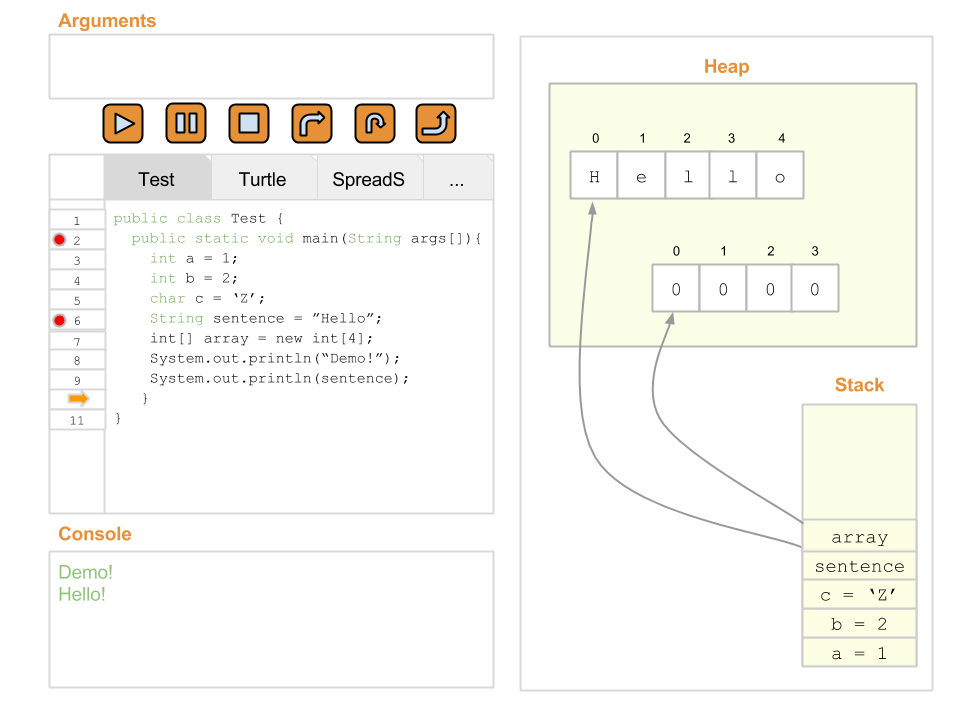
\includegraphics[height=70mm, width=60mm]{designIdea1.png}}
\quad
\subfigure[Second UI Design]{%
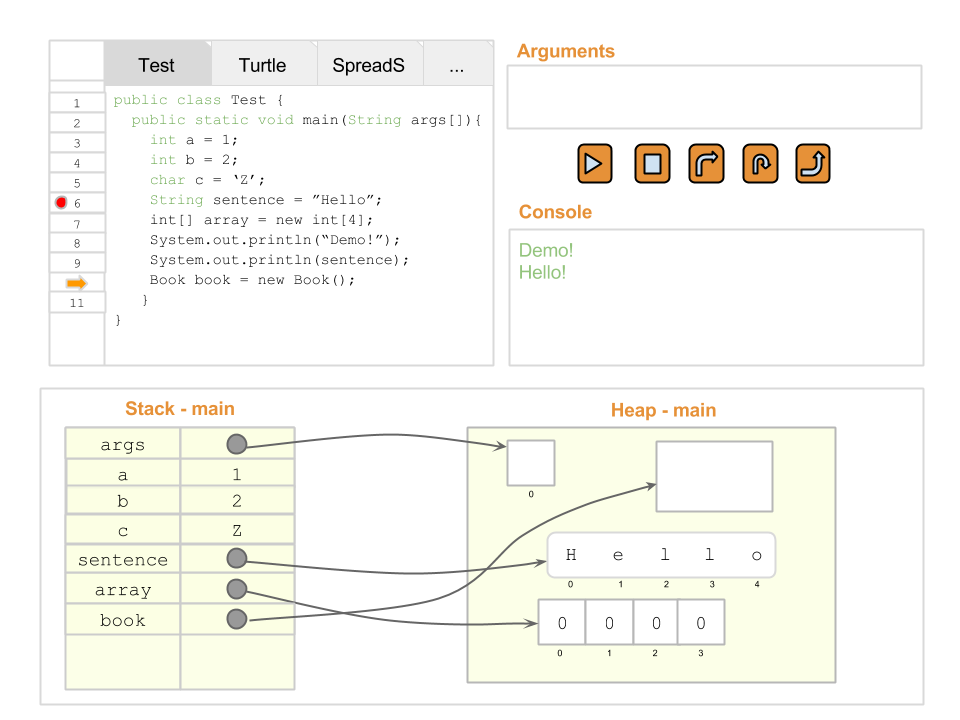
\includegraphics[height=70mm, width=60mm]{designIdea2.png}}
\end{figure}

Initially, we designed different views of the UI where the stack, heap and the code pane lay in different order.
After talking to Tristan, we thought if we put the stack and the heap visual at the bottom instead of on the right, we could better manage scenarios like small screens, a growing stack and large arrays.
As a result, we modified our UI design to be similar to the picture on the right above.\\
\begin{figure}[h!]
\centering
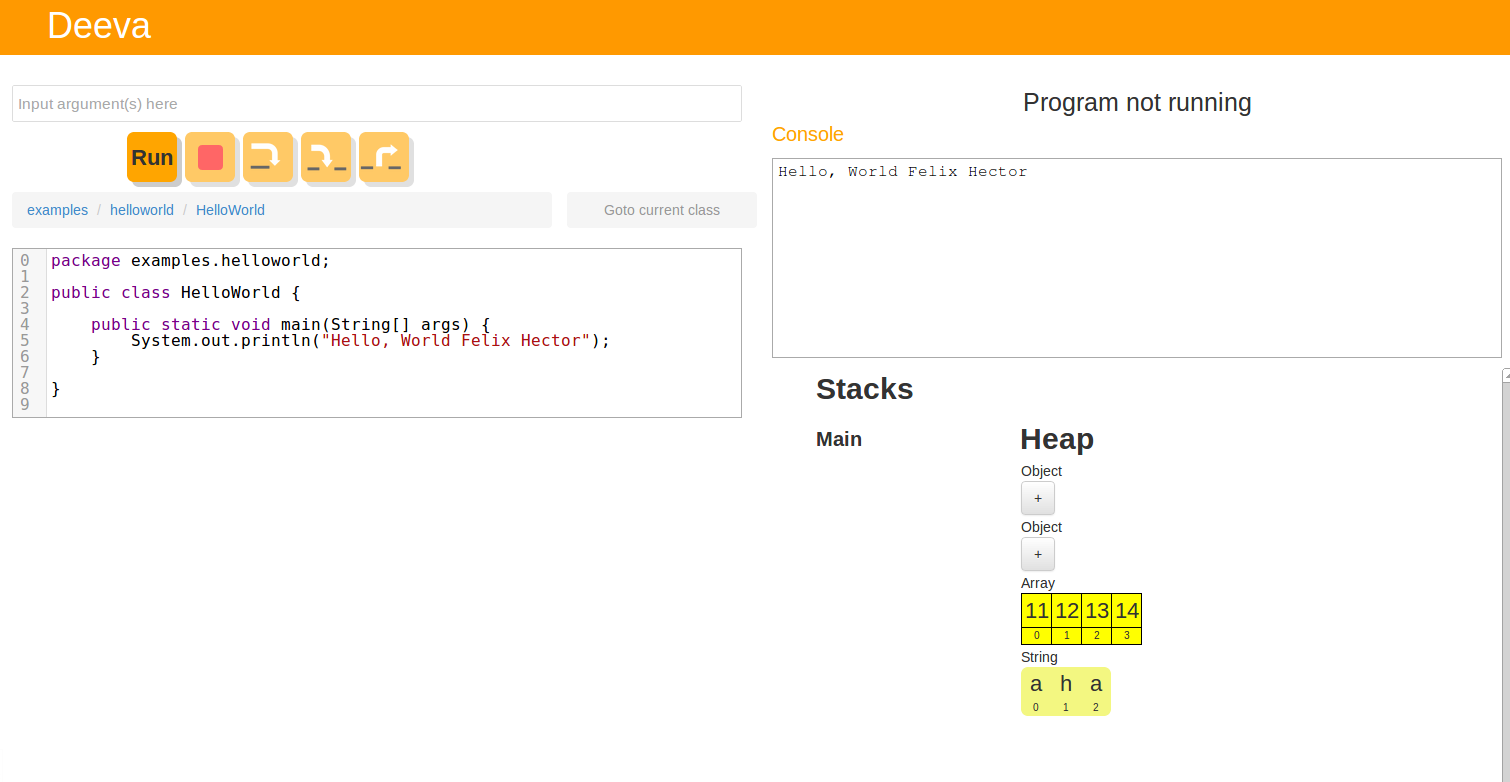
\includegraphics[height=70mm,width=130mm]{finalDesign.png}
\end{figure}

However, we thought if the stack grow more then eventually user would need to scroll up and down to be able to see the code and the stack and heap at the same time, which is not really what we want.
Therefore, we agreed on putting the stack and heap on the right with some modification to the first design.

\item[Button Design] \hfill \\
After interviews, we also found out that most of people find the naming and the design of buttons really confusing in Eclipse.
Especially “Step Into”, “Step Over” and “Step Return”. As a result, we designed several different sets of buttons and used a questionnaire to pick among them.
\begin{figure}[h!]
\centering

\includegraphics[height=20mm,width=60mm]{buttons1.png}
\end{figure}

This is the original design of “Stepping” buttons.
They inherit the design from Eclipse.
They are “Step Into”, “Step Over” and “Step Return” from left to right respectively. 

We asked one of our friends who is not from Computing and who has not used a debugger before what he thought they should do.
He could not quite figure out just by looking at them.
We then explained the concept of “Step Into”, “Step Over” and “Step Return” in terms of debugging and then asked again if he thought any of them really matched the buttons.
Some valuable feedback which we received from him was that: “It would be useful if we could somehow represent different scopes/lines so that the arrows (along with their direction) can correctly express the intended function.”
\begin{figure}[h!]
\centering

\includegraphics[height=20mm,width=60mm]{buttons2.png}
\end{figure}

This is our second design.
As suggested by our friend, the black lines indicate the lines of code which is similar to an editor. Arrows going in either the upwards or downwards directions indicate going to the next line, function, or (or previous) scope.
We created a questionnaire in which we explained the definition of “Next”, “Into” and “Out” (renamed as the previous ones weren’t completely intuitive).
Then we simply asked which of the eight button designs best represents the aforementioned functions.
We gave out the questionnaires when we did the Hallway Testing to some first year students and second year students.
Our second set of designs were much more popular than the original design on first year students.
However most of the second year students chose the original Eclipse design and one of them explained: “This is because we have already used Eclipse, and have known what step in, step out and step return are.”

However, at the end we did not use the second design because of some confusion raised by users and designers during the process. Some said that it is not that clear what the black lines indicate especially for experienced users who are already used to the original design.

\item[Colour Scheme and Font Size Design] \hfill \\
We carried out a questionnaire to see which colour scheme and font size are the most desirable one among the students. 
\begin{figure}[h!]
\centering
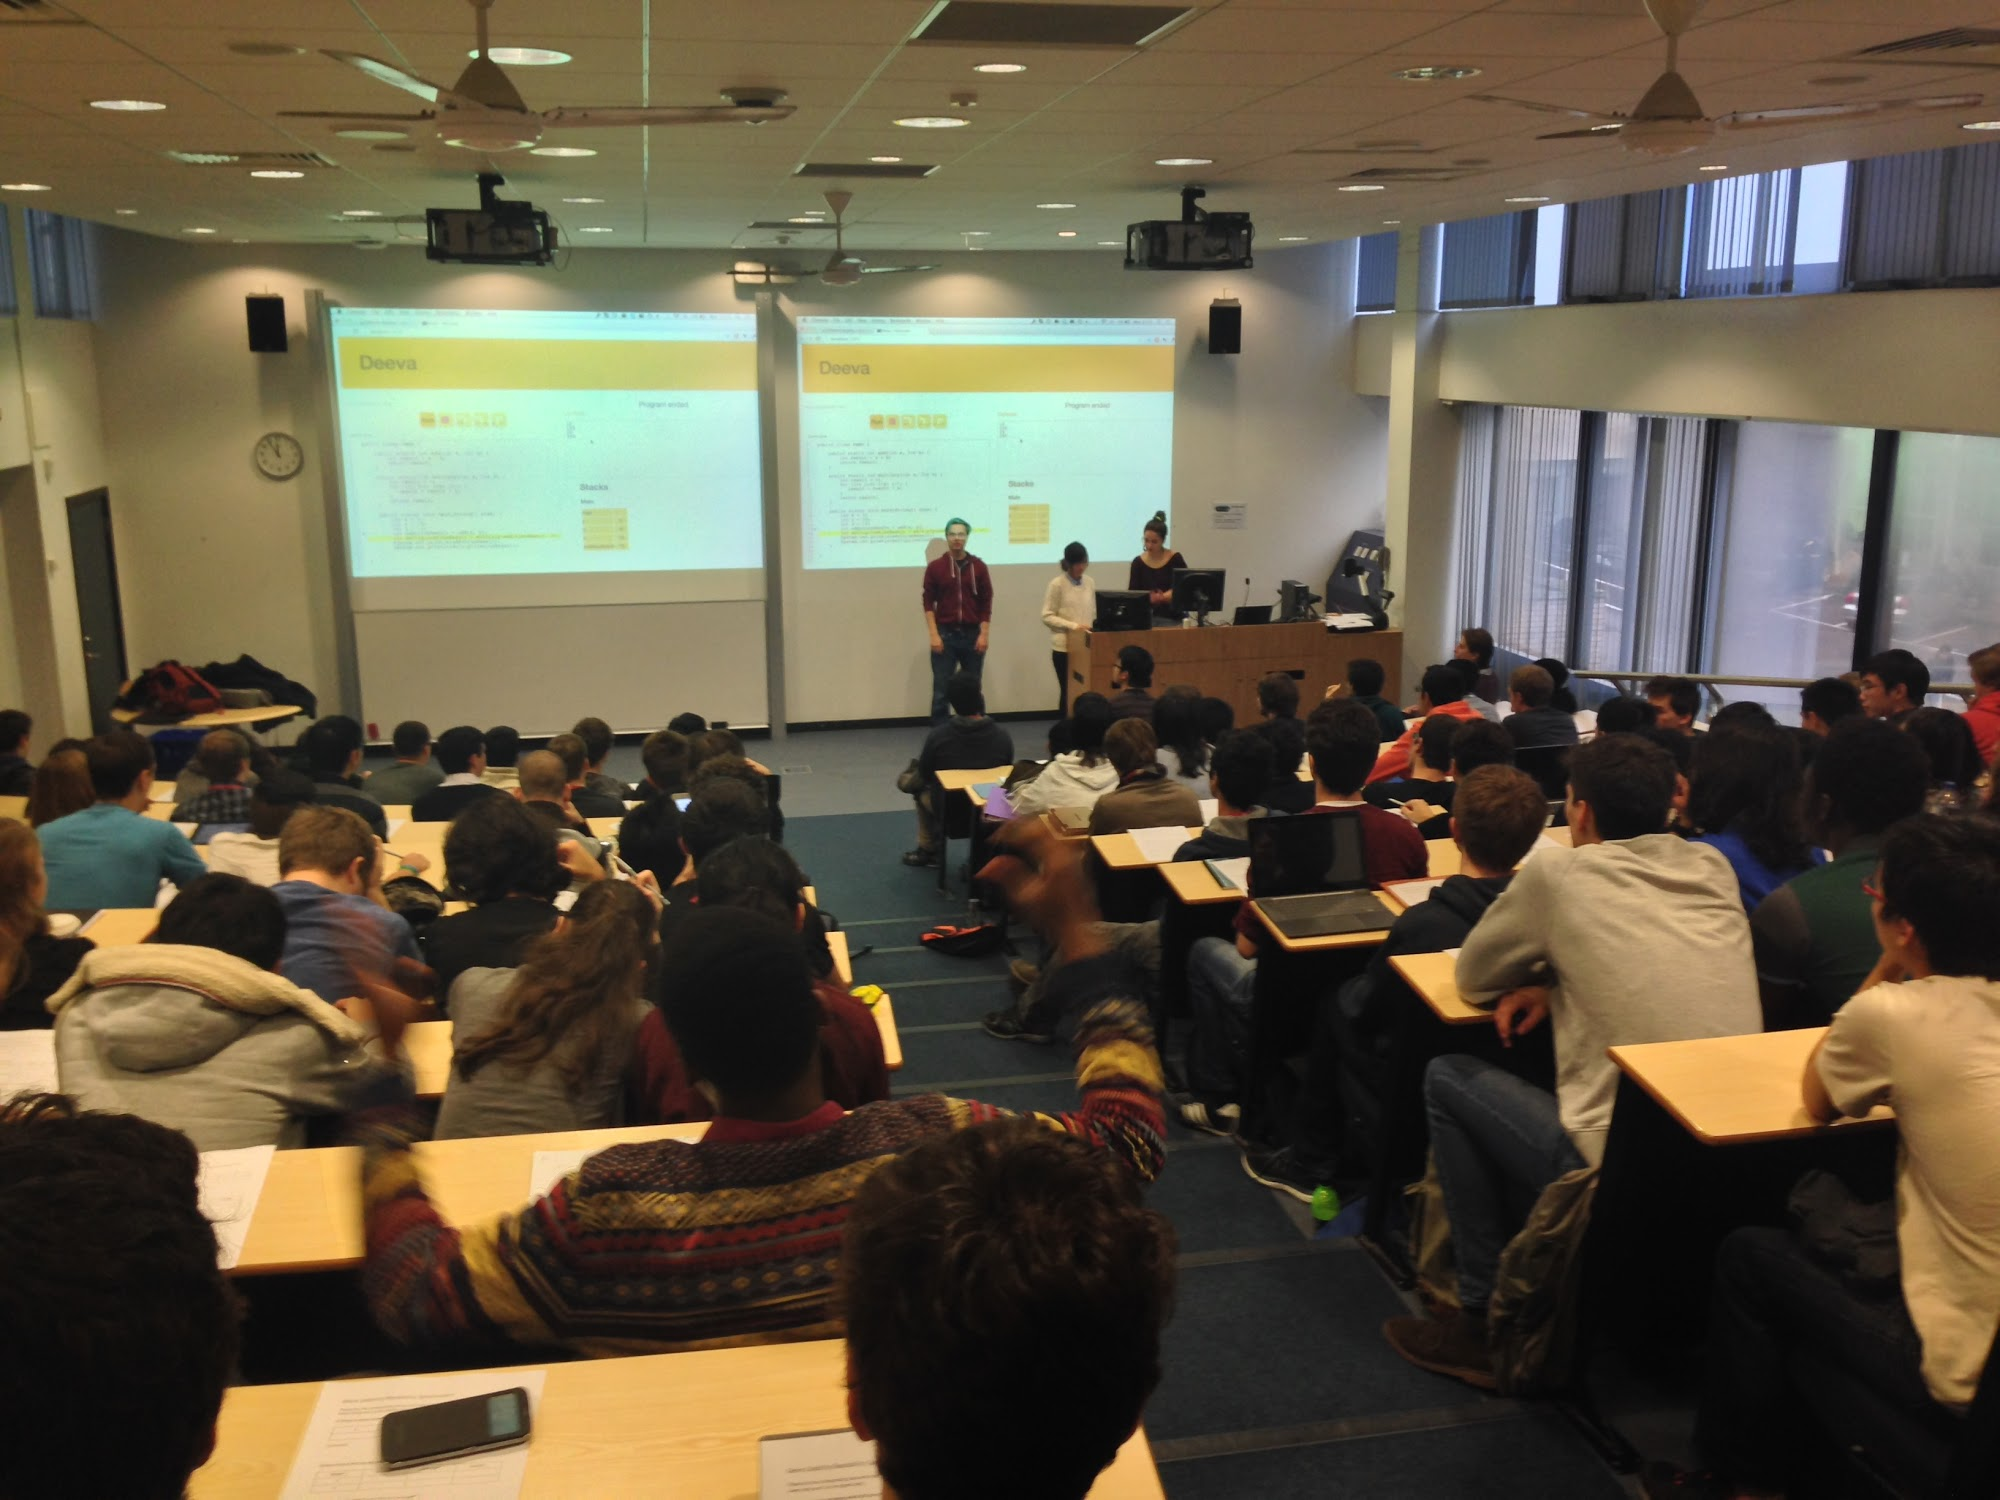
\includegraphics[height=50mm,width=100mm]{lectureHall.jpg}
\end{figure}

Given 5 different colour schemes, the preferred choice was our current colour scheme (orange), followed by a light blue color scheme (see graph on the right).
This validated our initial research that showed that in visual presentations, people are attracted to bright, warm colours that express optimism.
\begin{figure}[h!]
\centering
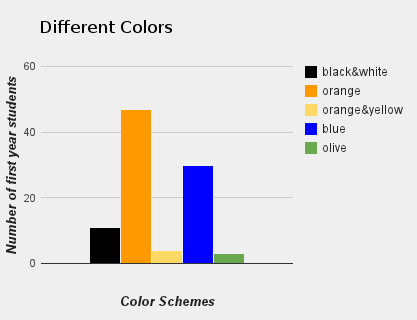
\includegraphics[height=60mm,width=100mm]{colours.png}
\end{figure}

As some people expressed that they would like the possibility to personalise Deeva and have a choice between different colour schemes we included this feature on the extended list of features for our final product.

However, this is not a priority as we are more concerned with implementing more functionality rather than a personalised UI design.

For font size, we provided 2 samples on the projector screen.
Sample 1 had a font size of 26px and Sample 2 had a font size of 16px.
\begin{figure}[h!]
\centering
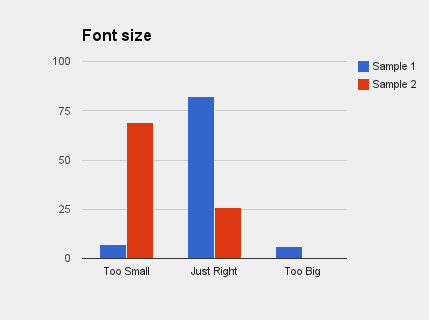
\includegraphics[height=60mm,width=100mm]{fonts.png}
\end{figure}
As this questionnaire was performed in one of the big lecture rooms (Huxley 311) the results for this question did not surprise us, ie. people preferred the sample with the bigger font size (see graph on the right).
However, as the smaller font size sample is perfectly readable on the lab machines we are thinking of releasing our debugger in two modes: ‘normal mode’ (to be used on the lab machines - font size 16) and  ‘lecturer mode’ (to be used by lecturers when teaching - font size 26).
This was not part of our initial plan but we currently added creating a ‘lecturer mode’ to the top of our list of extensions.

\end{description}
\subsection{System Design}

\section{Implementation}
\subsection{Technology Evaluation}
\subsection{Overview}
\subsection{Details}
\subsubsection{Front End}
\subsubsection{Middleware}
\subsubsection{Back End}

\section{Evaluation}
\subsection{Testing}

\section{Project Management}
\subsection{Team Member Contributions}
\subsubsection{Kritaphat Sonsri-in}
\subsubsection{Xueqi Chen}
\subsubsection{Alina Draganescu}
\subsubsection{Felix de Souza}
\subsubsection{Hector Dearman}
\subsection{Team Management}

To ensure effective development of the product, weekly supervisor meetings were scheduled.
In these meetings, quality assurance was the main aim, making sure we were on the right track with our development, delivering correct features. 
This avoided unnecessary misunderstandings and extra time spent on creating unneeded features for the product. 

Further to the supervisor meetings, weekly group meetings ensured that all group members are in sync about the progress and direction of the project. 
During these meetings, the information gathered from the supervisor meetings would be recapped and the targets for the upcoming week would be set. 
Thus, tasks could be divided among group members, with everyone knowing what their colleagues are working on in this week, making group and individual efforts significantly more effective.
\begin{figure}[h!]
\centering
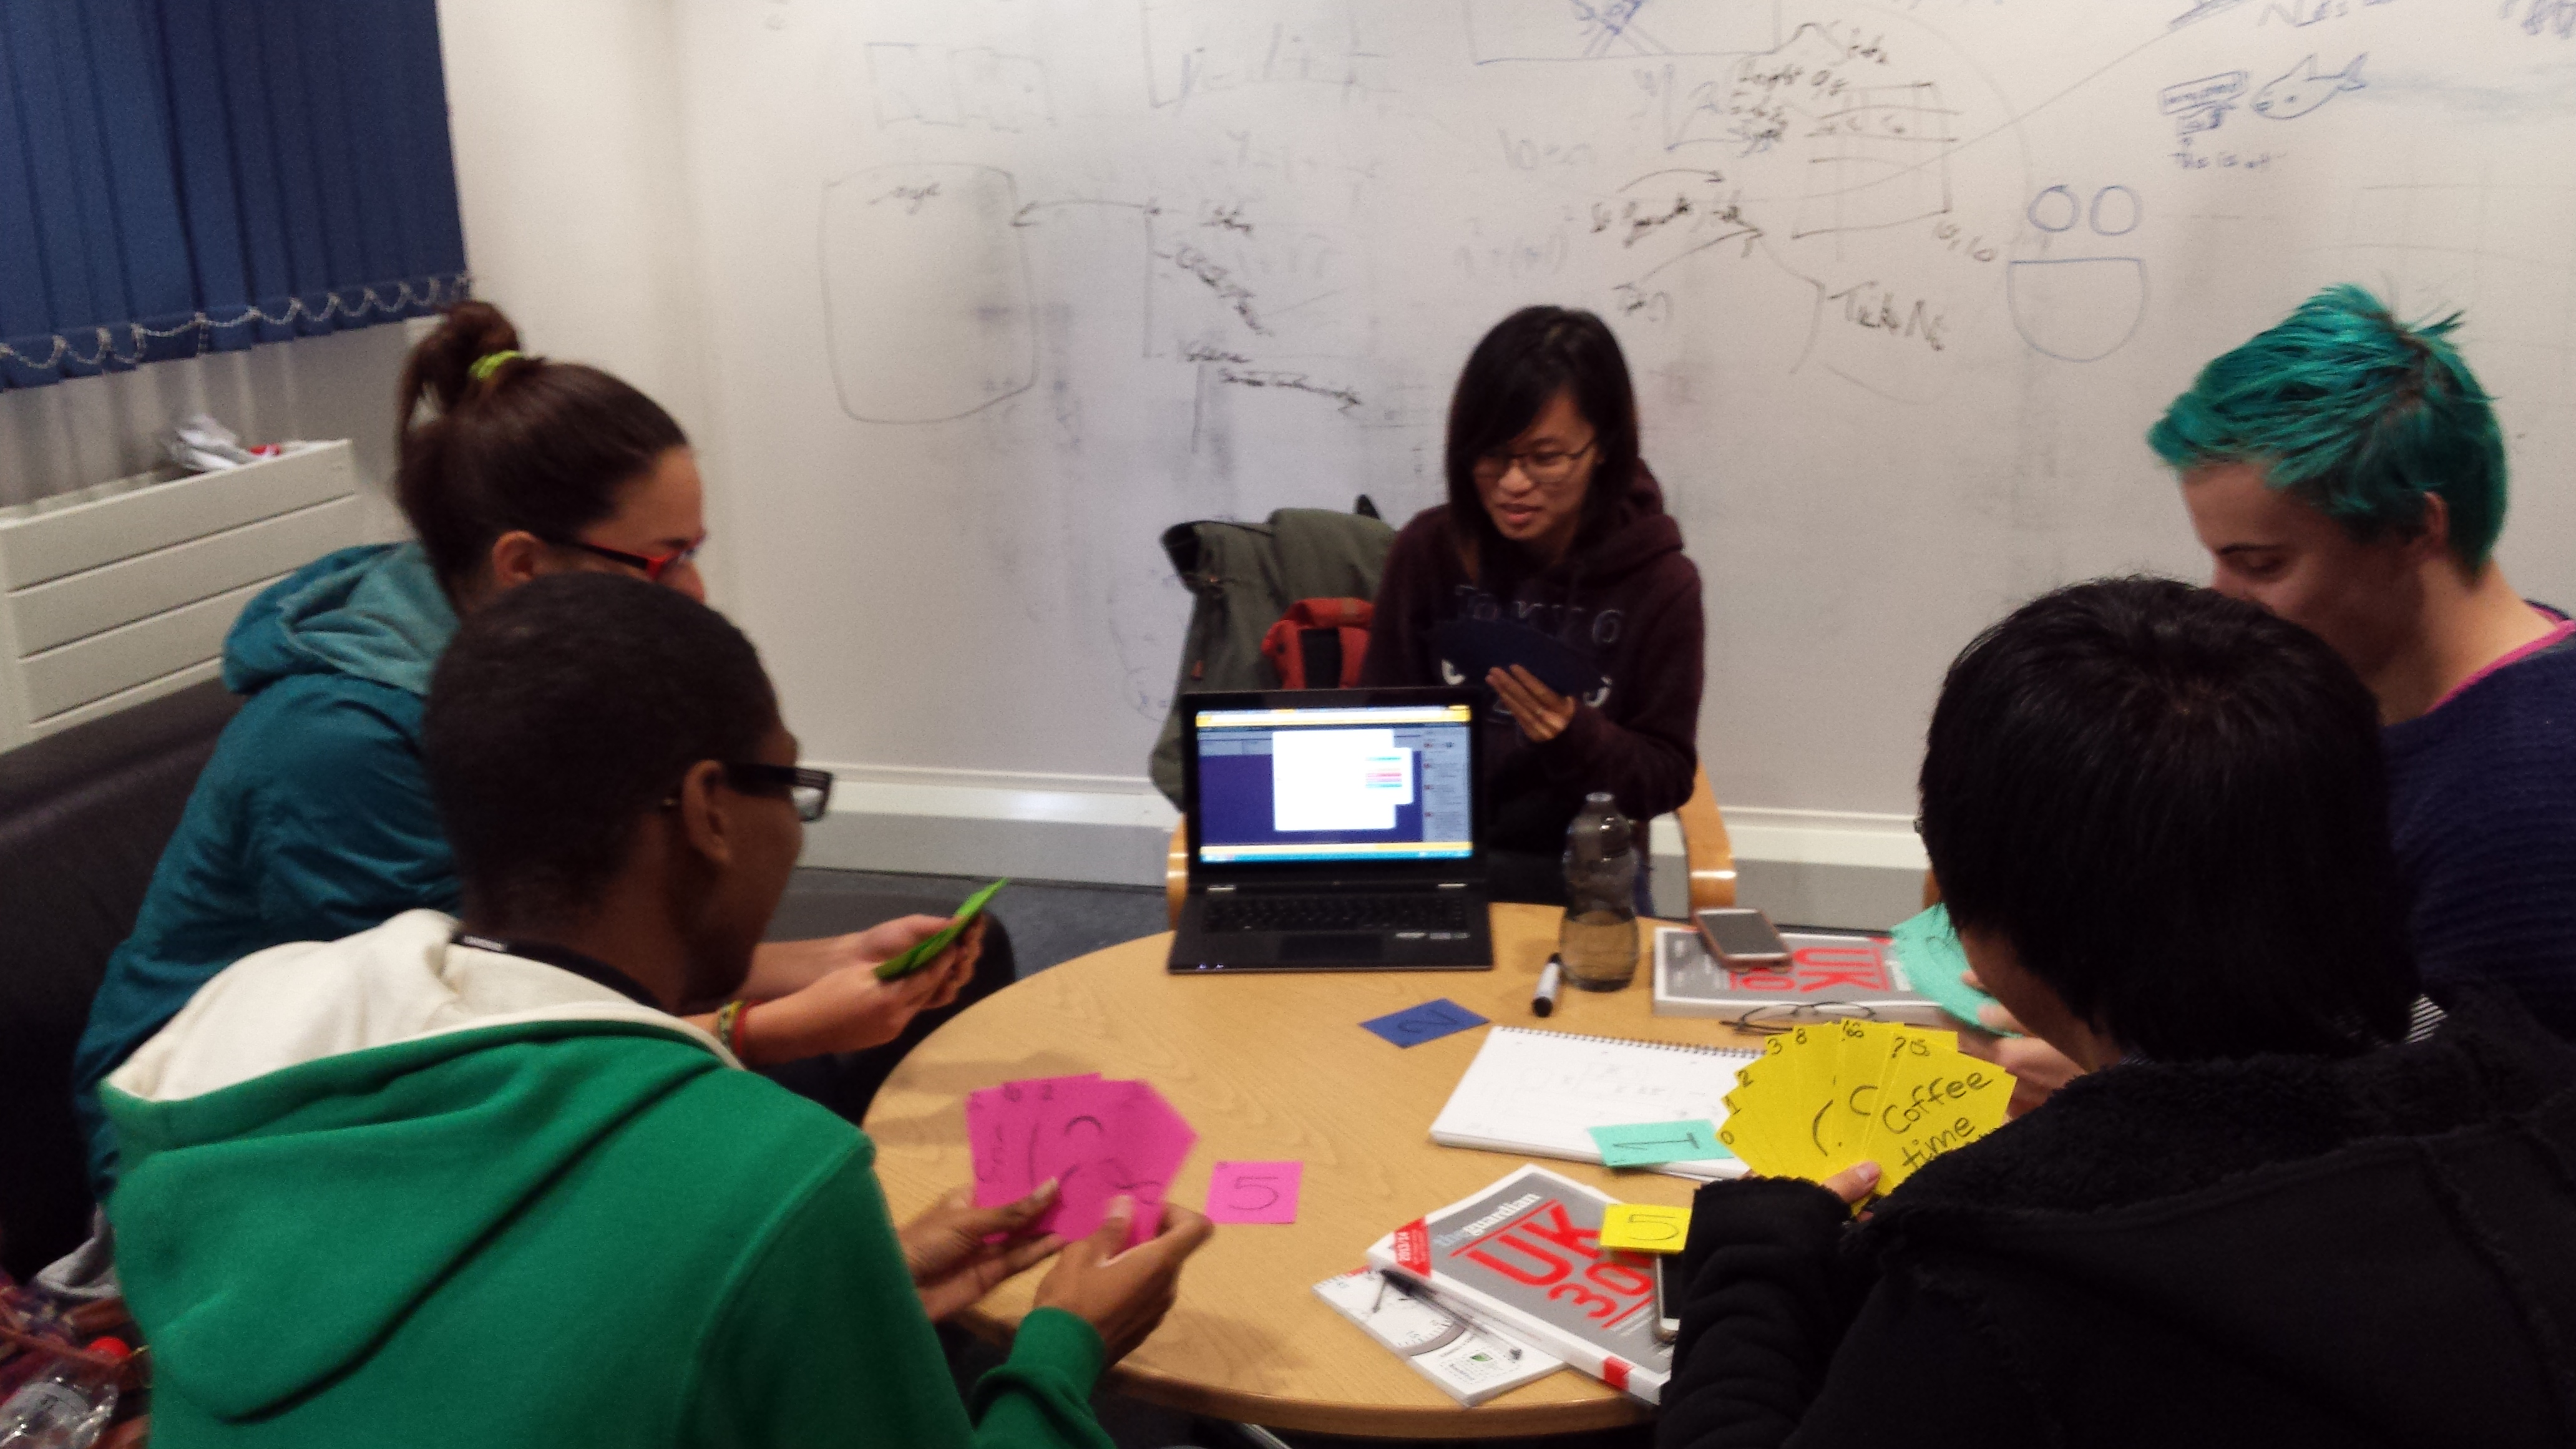
\includegraphics[height=80mm,width=130mm]{estimation.jpg}
\end{figure}

To aid the management of the project on a holistic and timely perspective, several tools were used, which will be outlined in the following section.

\subsection{Tools}
\begin{description}

\item[Trello] \hfill \\
\begin{figure}[h!]
\centering
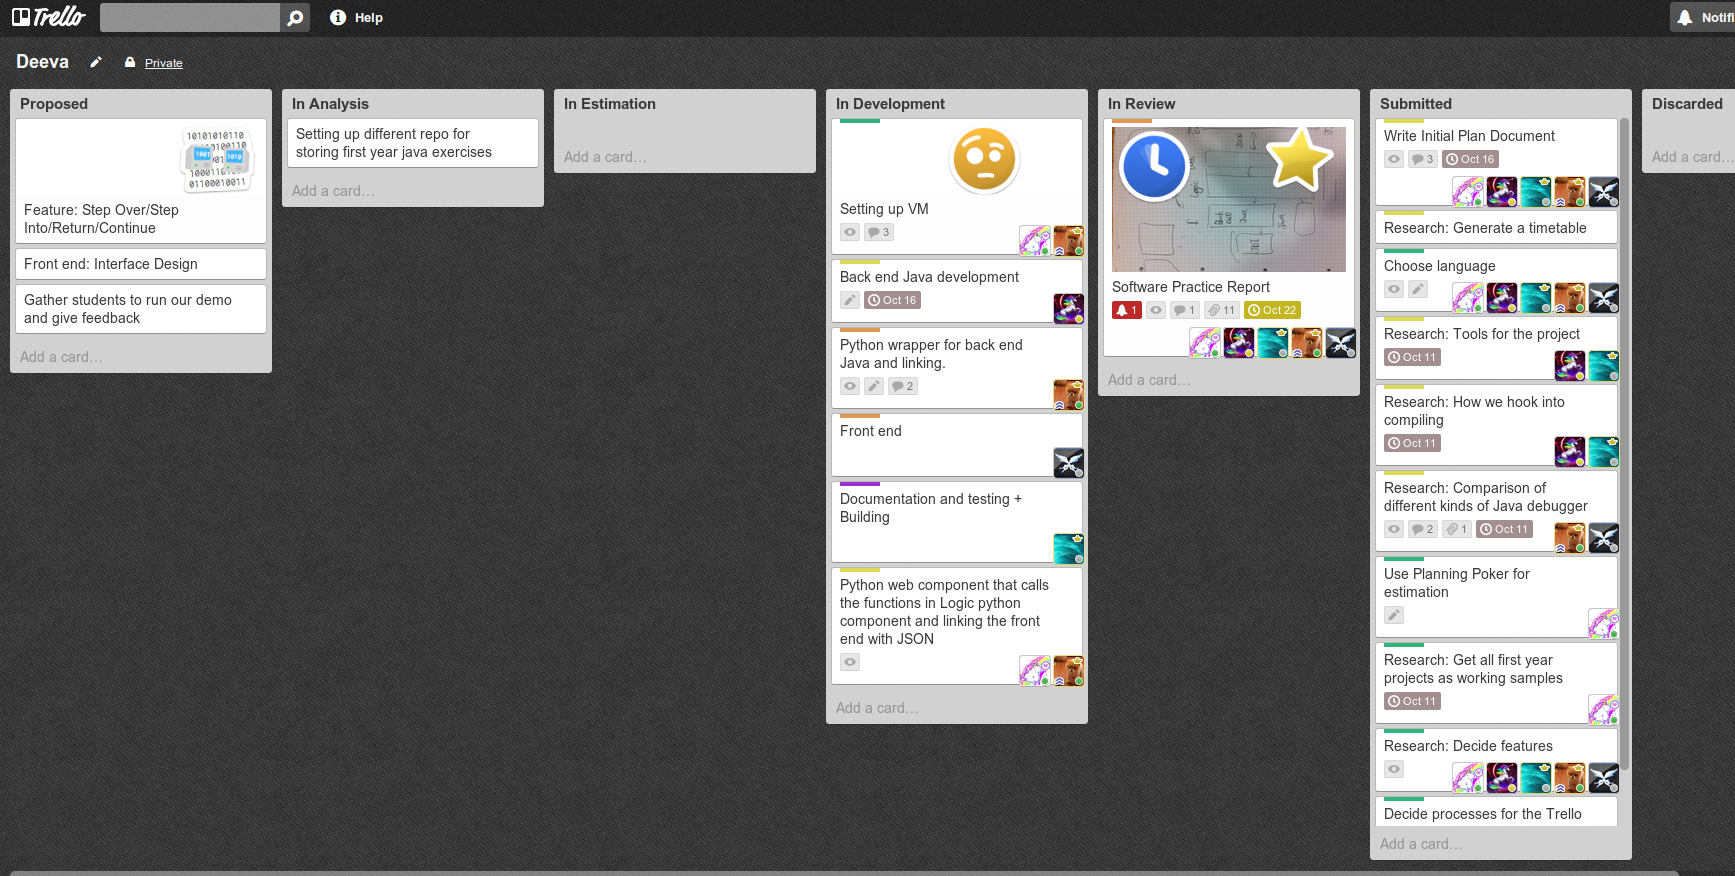
\includegraphics[height=80mm,width=130mm]{Trello.png}
\end{figure}

We used Trello as our project management tool and as an Information Radiator\footnote{\tt{https://www.atlassian.com/wallboards/information-radiators.jsp}}.
It also allows us to track our progress and average velocity. 
We decided to use Trello as it fulfills most of the key features required for such a tool: it is easy to use and update, relatively flexible and allows for communications between members without too much interruption. 
We decided to use an electronic version as they are a more manageable alternative to physical boards. 
We also found it extremely useful when it came to keeping everyone informed on the general progress and keeping all the information in one compact environment.

A Trello board was created for a better project management process. 
There are several different swimlanes on the board: ``Proposed'', which allows all members to throw in ideas; ``In Analysis'', where people talk about their ideas and have a discussion with group members to see if the story is feasible. 
If it is, the card will be then moved to ``In Estimation'' where we would use Planning Poker to assign the story with a complexity points.
Otherwise, the story will be moved to ``Discarded''.
The reason why we want to keep track of what we have discarded is that we might have thought we would not have time for it, but in reality we may have time at the end.
We might want to move it back and reconsider it. 
After ``In Estimation'', the card will be assigned to group members with a set due date and be moved into ``In Development'' on the Trello board. 
Once the development is complete, the card should be moved into ``In Review''. 
This is when we meet as a group and review our code to improve our style and pattern-usage.

\item[Planing Poker] \hfill \\
\begin{figure}[h!]
\centering
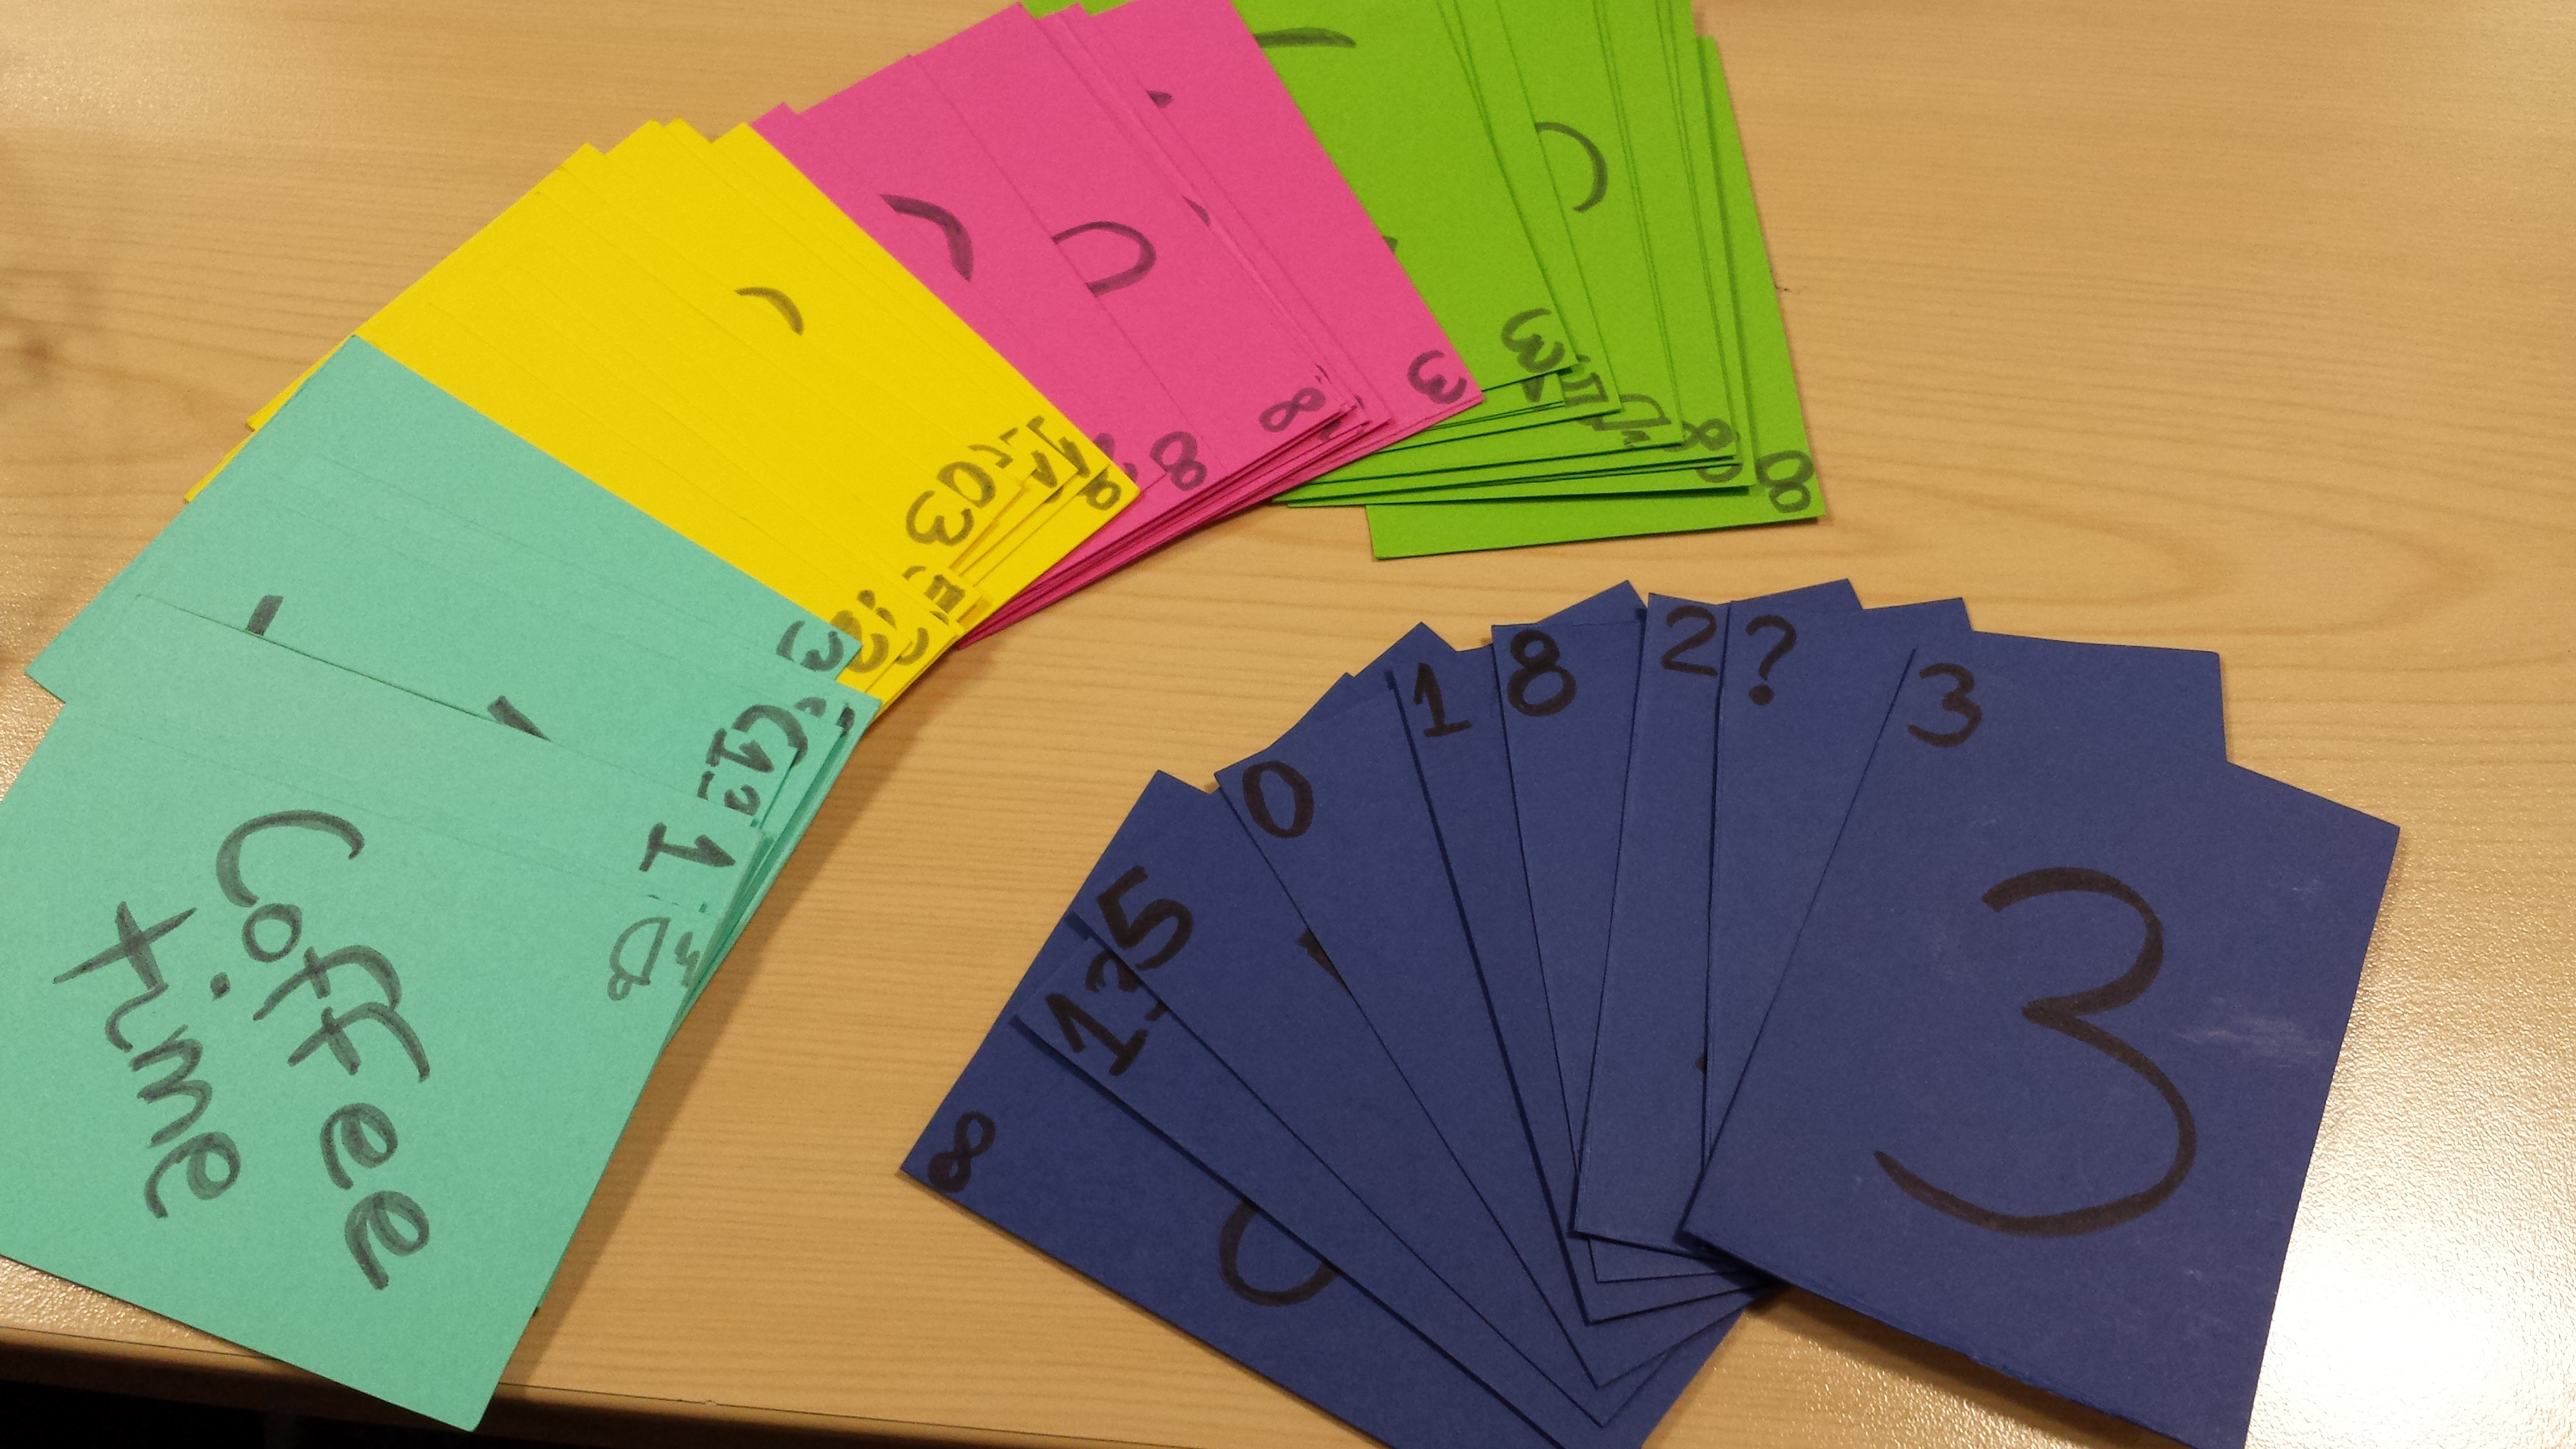
\includegraphics[height=80mm,width=130mm]{planningPokers.jpg}
\end{figure}

We are using Planning Poker in order to estimate stories in each cycle of development. 
This method is known to avoid anchoring and will produce more accurate, less optimistic story point estimations\footnote{\tt{http://en.wikipedia.org/wiki/Planning\_poker\#Planning\_poker\_benefits}}. This technique takes some time to get used to because initially the story point bared little meaning to us.
As we estimated more tasks, the story points became more meaningful hence the poker game proved to be a very efficient method.

For example, it helped determine when people aren't really talking about the same scope for a certain task.
Frequently we have a task like ``Set up the back end." and one person gives a task a 2 while another gives it an 8.
The first person thinks the task title means ``Write some stubs so the middleware can integrate." while the second thinks it means ``Implement the backend up to the minimal specification.". 
So using planing poker has already helped us make sure we're all on the same page.
One of our group members hand-made a set of poker cards just for estimation.
It contains the Fibonacci numbers up to 13 including 0 and infinity - if the task was unfeasible in the time given, as well as ``coffee time'' if we think we needed a break. 

\item[Facebook Group] \hfill \\
Creating a Facebook group proved very efficient for communicating meeting times and general enquiries that were too conversational for Trello.  

\item[Google Docs] \hfill \\
We used Google Docs for collaborative editing on reports, plans and meeting summaries in real time.
  
\item[Github] \hfill \\
Github is a hosted source control which somebody else manages and is easily accessible from anywhere and also plays nicely with the hosted Continuous Integration tool - Travis CI\footnote{\tt{http://travis-ci.com/}}.

\item[Travis CI] \hfill \\
\todo{about Travis here}
\end{description}

\section{Extensions}
\section{Conclusion}

\clearpage
\thispagestyle{empty}
\null\vfill
\begin{center}
\settowidth\longest{``A process cannot be understood by stopping it."}
\parbox{\longest}{%
  \raggedright{%
  ``A process cannot be understood by stopping it." \\
  }   
  \raggedright{\emph{First Law of the Mentat -- Dune}}\par%
}
\end{center}
\addcontentsline{toc}{section}{Quote}
\vfill\vfill
\clearpage

\appendix
\section{Initial Plan}
\label{sec:initialplan}
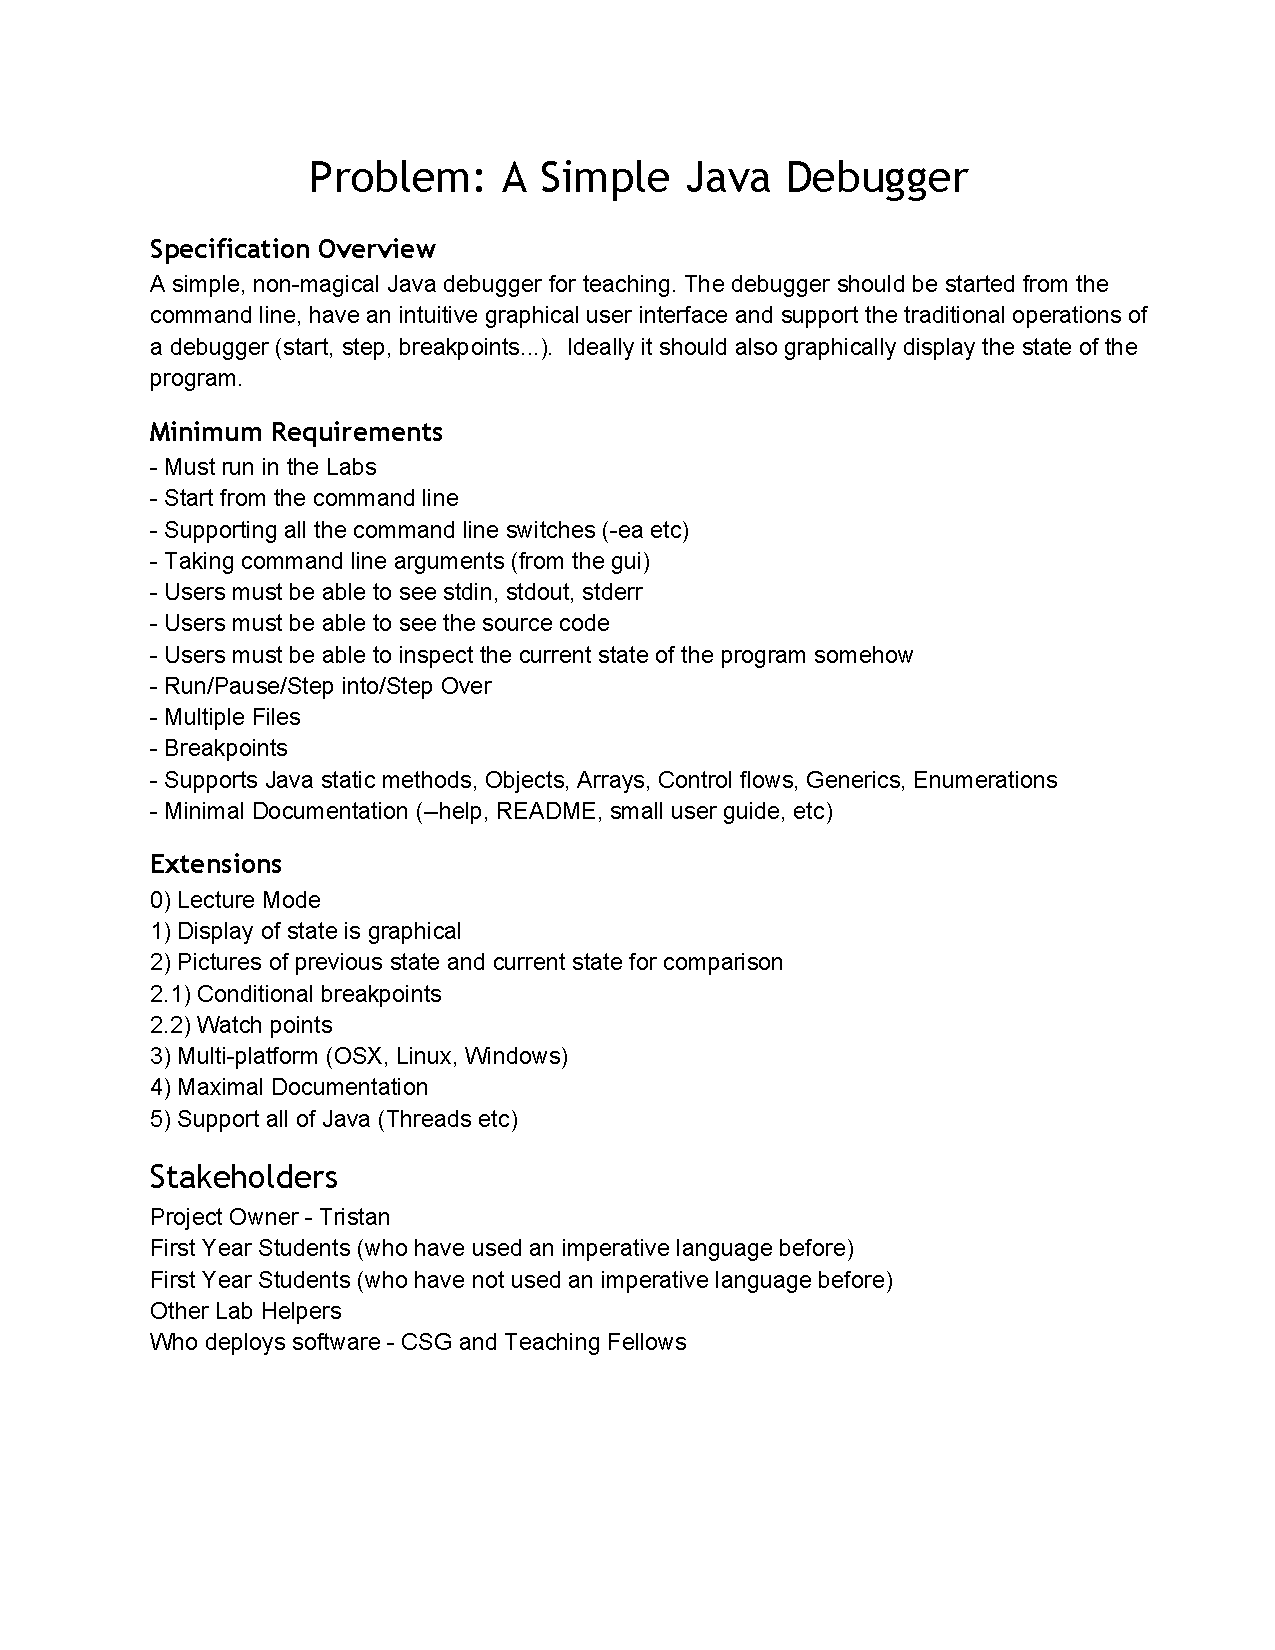
\includepdf[pages={-}, pagecommand={}]{plan.pdf}

\end{document}
